%%%%%%%%%%%%%%%%%%%%%%%%%%%%%%%%%%%%%%%%%%%%%%%%%%%%%%
%%%%%%%%%%%%%%%%%%%%%%%%%%%%%%%%%%%%%%%%%%%%%%%%%%%%%%%%%%%%%%%%%%%%
\def\scl{1}%scaling factor of the picture


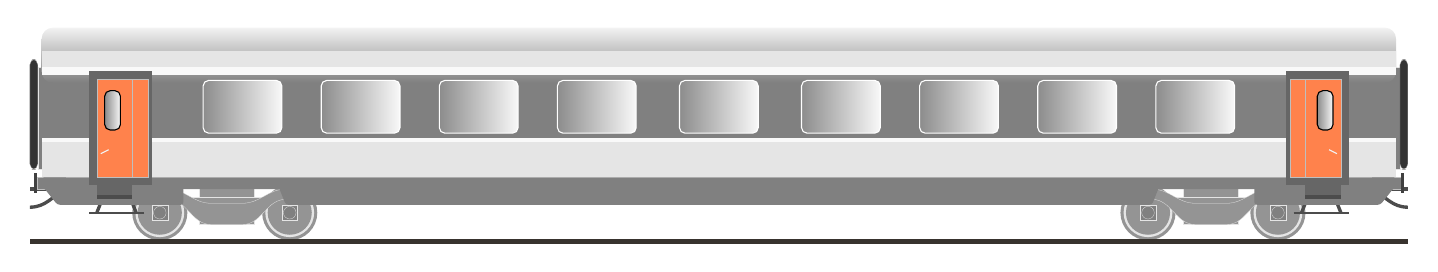
\begin{tikzpicture}[
  scale=\scl,
  %wagon/.style={yellow!30!brown!20!,rounded corners,draw=black,thick},
  wagon/.style={green!70!brown!20!black!75!,draw=black,thick},
 % toit/.style={black!70!brown!20!,draw=gray,thick},
  %roue/.style={brown!20!black!70!,draw=black,thick},
  fenetre/.style={white,rounded corners = 2pt,draw=black, thick},
  porte/.style={color=red!70!yellow!70!,draw=gray!50!, ultra thin}
  ]

  \begin{scope}[xshift=0 cm,yshift=0 cm]%, scale = 0.3
%
%         LIAISONS
% 
  \fill[color=gray,draw=gray!20!, ultra thin] % souflet gris
 (8.65, 0.9) rectangle (-8.65, 2.2);

 \draw[black!70!, very thick] 
    (8.3,0.65) to[out=330,in=180] (8.75,0.42);
 \draw[black!70!, very thick] 
    (-8.3,0.65) to[out=210,in=0] (-8.75,0.42);

  \foreach \t in {-1, 1}
  {
  \fill[color=black!80!,draw=gray!80!, ultra thin, rounded corners=2pt] % 
 (8.65 * \t, 0.9) rectangle (8.75 * \t, 2.3); % gris foncé, souflet

    \coordinate (A) at (8.3 * \t,0.65) ;
    \coordinate (B) at (8.75 * \t,0.65) ;
 \draw[black!70!, ultra thick] 
    (A) -- (B);

  }

 % BUTOIRS
  \foreach \t in {-1, 1}
  {
  \fill[color=gray,draw=gray!50!, ultra thin] % 
 (8.3 * \t, 0.65) rectangle (\t * 8.66, 0.8);
  \fill[color=gray!50!black] % 
 (\t * 8.66, 0.6) rectangle (\t * 8.7, 0.85);
  }
%
%     CORPS DU WAGON
%
  \shade[bottom color=gray, top color=gray!10!, rounded corners]  % toit
 (-8.6, 2) rectangle (8.6, 2.7);

  \fill[color=gray!20!] % gris clair
 (-8.6, 2.1) rectangle (8.6, 2.4);
  \fill[color=gray!20!] % gris clair
 (-8.6, 0.8) rectangle (8.6, 1.25);

  \fill[color=gray!5!] % blanc
 (-8.6, 2.1) rectangle (8.6, 2.2);
  \fill[color=gray!5!] % blanc
 (-8.6, 1.25) rectangle (8.6, 1.3);


% Arriere roues
  %\foreach \x in {6.25, -6.25} \fill[brown!40!black] (\x - 0.85, 0.8) rectangle (\x + 0.85, 0.45);

%  ROUES
\def\hauteur{0.35}% de l'axe des roues
\tikzset{
  roue/.pic={
    \fill[black!20!gray!70!] (0, \hauteur) circle (0.35 cm);
    \fill[gray!20!] (0, \hauteur) circle (0.31 cm);
    \fill[black!20!gray!70!] (0, \hauteur) circle (0.28 cm);

  \fill[color=gray,draw=gray!20!, ultra thin] %,rotate=45
 (0.1, \hauteur + -0.1) rectangle (-0.1, \hauteur + 0.1);

  \fill[color=gray,draw=gray!20!, ultra thin] (0, \hauteur) circle (0.08 cm);

  }
}

  \pic at (5.45,0)    {roue};
  \pic at (7.1,0)    {roue};
  \pic at (-5.45,0)    {roue};
  \pic at (-7.1,0)    {roue};
 % ESSIEUX
\def\y{0.2}
  \foreach \x in {6.25, -6.25}
   {
 \fill[black!20!gray!70!,draw=gray!20!, ultra thin] 
  (\x - 0.35, 0.2) rectangle (\x + 0.35, 0.45);

 \fill[black!20!gray!70!,draw=gray!20!, ultra thin] 
  (\x - 0.45, 0.45) rectangle (\x + 0.45, 0.55);

 \fill[black!20!gray!70!,draw=gray!20!, ultra thin] 
  (\x - 0.35, 0.55) rectangle (\x + 0.35, 0.7);

    \coordinate (A) at (\x + -0.75,\y + 0.45) ;
      \coordinate (B) at (\x - 0.2,\y + 0.27) ;
      \coordinate (C) at (\x + 0.2,\y + 0.27) ;
    \coordinate (D) at (\x + 0.75,\y + 0.45) ;
    \coordinate (E) at (\x + 0.75,\y + 0.32) ;
      \coordinate (F) at (\x + 0.2,\y + 0) ;
      \coordinate (G) at (\x - 0.2,\y + 0) ;
    \coordinate (H) at (\x - 0.75,\y + 0.32) ;
 \fill[black!20!gray!70!,draw=gray!20!, ultra thin] 
    (A) to[out=0,in=180] (B) to[out=0,in=180] (C) to[out=0,in=180]
    (D) to[out=-90,in=90] (E) to[out=180,in=0] (F) to[out=180,in=0]
    (G) to[out=180,in=0] (H) -- cycle;
  }

% MARCHE
  \foreach \t in {-1, 1}
  {
    \draw[draw=black!70!,very thick] % montant
 (\t * 7.9, 0.35) -- (\t * 7.8, 0.6);
    \draw[draw=black!70!,very thick] % montant
 (\t * 7.4, 0.35) -- (\t * 7.5, 0.6);
    \draw[draw=black!70!,thick] % marche
 (\t * 7.3, 0.35) -- (\t * 8, 0.35);
  }

% BAS DE CAISSE

  \fill[color=gray, rounded corners=1pt] % gris Foncé
    (-8.6, .8) rectangle (8.6, .65);


  \foreach \t in {-1, 1}
  \fill[color=gray, rounded corners=1pt] % gris Foncé
    (\t * 8.6, .7) -- (\t * 8.4, .45) -- (\t * 6.8, .45) -- (\t * 6.8, .7) -- cycle;
  \fill[color=gray, rounded corners=1pt] % gris Foncé
    (5.6, .7) -- (5.5, .45) -- (-5.5, .45) -- (-5.6, .7) -- cycle;

      % FENÊTRES
  \foreach \t in {1.05, 2.55, 4.05, 5.55}
  {
  \shade[bottom color=gray!5!, top color=gray!90!, shading angle={90},rounded corners=2pt, draw=white]
   (\t, 1.36) rectangle (\t + 1, 2.03);
  \shade[bottom color=gray!5!, top color=gray!90!, shading angle={90},rounded corners=2pt, draw=white]
   (-\t, 1.36) rectangle (-\t - 1, 2.03);
  }
  \shade[bottom color=gray!5!, top color=gray!90!, shading angle={90},rounded corners=2pt, draw=white]
   (-0.5, 1.36) rectangle (0.5, 2.03);

      % PORTES
  \foreach \t in {-1, 1}
  {

    \fill[gray!80!black] % marche
 (\t * 7.45, 0.53) rectangle (\t * 7.9, 0.7);
    \fill[gray!60!black] % marche
 (\t * 7.45, 0.53) rectangle (\t * 7.9, 0.57);

  \fill[gray!80!black]
 (\t * 7.2, 0.7) rectangle (\t * 8, 2.15);
  \fill[porte]
 (\t * 7.25, 0.8) rectangle (\t * 7.6, 2.05);
  \fill[porte]
 (\t * 7.45, 0.8) rectangle (\t * 7.9, 2.05);

  \shade[bottom color=gray!5!, top color=gray!90!, shading angle={90},rounded corners=2pt, draw=black] % fenêtre
   (\t * 7.6, 1.4) rectangle (\t * 7.8, 1.9);

    \draw[gray!10!]
 (\t * 7.75, 1.15) -- (\t * 7.85, 1.1); % poignée
  }

  % RAIL
  \fill[color=brown!20!gray!40!black]
 (-8.75, 0.02) rectangle (8.75, -0.05);

  \end{scope}
%
%
\end{tikzpicture}
%
